%!TEX TS-program = xelatex

% Шаблон документа LaTeX создан в 2018 году
% Алексеем Подчезерцевым
% В качестве исходных использованы шаблоны
% 	Данилом Фёдоровых (danil@fedorovykh.ru) 
%		https://www.writelatex.com/coursera/latex/5.2.2
%	LaTeX-шаблон для русской кандидатской диссертации и её автореферата.
%		https://github.com/AndreyAkinshin/Russian-Phd-LaTeX-Dissertation-Template

\documentclass[a4paper,14pt]{article}


%%% Работа с русским языком
\usepackage[english,russian]{babel}   %% загружает пакет многоязыковой вёрстки
\usepackage{fontspec}      %% подготавливает загрузку шрифтов Open Type, True Type и др.
\defaultfontfeatures{Ligatures={TeX},Renderer=Basic}  %% свойства шрифтов по умолчанию
\setmainfont[Ligatures={TeX,Historic}]{Times New Roman} %% задаёт основной шрифт документа
\setsansfont{Comic Sans MS}                    %% задаёт шрифт без засечек
\setmonofont{Courier New}
\usepackage{indentfirst}
\frenchspacing

\renewcommand{\epsilon}{\ensuremath{\varepsilon}}
\renewcommand{\phi}{\ensuremath{\varphi}}
\renewcommand{\kappa}{\ensuremath{\varkappa}}
\renewcommand{\le}{\ensuremath{\leqslant}}
\renewcommand{\leq}{\ensuremath{\leqslant}}
\renewcommand{\ge}{\ensuremath{\geqslant}}
\renewcommand{\geq}{\ensuremath{\geqslant}}
\renewcommand{\emptyset}{\varnothing}

%%% Дополнительная работа с математикой
\usepackage{amsmath,amsfonts,amssymb,amsthm,mathtools} % AMS
\usepackage{icomma} % "Умная" запятая: $0,2$ --- число, $0, 2$ --- перечисление

%% Номера формул
%\mathtoolsset{showonlyrefs=true} % Показывать номера только у тех формул, на которые есть \eqref{} в тексте.
%\usepackage{leqno} % Нумерация формул слева	

%% Перенос знаков в формулах (по Львовскому)
\newcommand*{\hm}[1]{#1\nobreak\discretionary{}
	{\hbox{$\mathsurround=0pt #1$}}{}}

%%% Работа с картинками
\usepackage{graphicx}  % Для вставки рисунков
\graphicspath{{images/}}  % папки с картинками
\setlength\fboxsep{3pt} % Отступ рамки \fbox{} от рисунка
\setlength\fboxrule{1pt} % Толщина линий рамки \fbox{}
\usepackage{wrapfig} % Обтекание рисунков текстом

%%% Работа с таблицами
\usepackage{array,tabularx,tabulary,booktabs} % Дополнительная работа с таблицами
\usepackage{longtable}  % Длинные таблицы
\usepackage{multirow} % Слияние строк в таблице
\usepackage{float}% http://ctan.org/pkg/float

%%% Программирование
\usepackage{etoolbox} % логические операторы


%%% Страница
\usepackage{extsizes} % Возможность сделать 14-й шрифт
\usepackage{geometry} % Простой способ задавать поля
\geometry{top=20mm}
\geometry{bottom=20mm}
\geometry{left=20mm}
\geometry{right=10mm}
%
%\usepackage{fancyhdr} % Колонтитулы
% 	\pagestyle{fancy}
%\renewcommand{\headrulewidth}{0pt}  % Толщина линейки, отчеркивающей верхний колонтитул
% 	\lfoot{Нижний левый}
% 	\rfoot{Нижний правый}
% 	\rhead{Верхний правый}
% 	\chead{Верхний в центре}
% 	\lhead{Верхний левый}
%	\cfoot{Нижний в центре} % По умолчанию здесь номер страницы

\usepackage{setspace} % Интерлиньяж
\onehalfspacing % Интерлиньяж 1.5
%\doublespacing % Интерлиньяж 2
%\singlespacing % Интерлиньяж 1

\usepackage{lastpage} % Узнать, сколько всего страниц в документе.

\usepackage{soul} % Модификаторы начертания

\usepackage{hyperref}
\usepackage[usenames,dvipsnames,svgnames,table,rgb]{xcolor}
\hypersetup{				% Гиперссылки
	unicode=true,           % русские буквы в раздела PDF
	pdftitle={Заголовок},   % Заголовок
	pdfauthor={Автор},      % Автор
	pdfsubject={Тема},      % Тема
	pdfcreator={Создатель}, % Создатель
	pdfproducer={Производитель}, % Производитель
	pdfkeywords={keyword1} {key2} {key3}, % Ключевые слова
	colorlinks=true,       	% false: ссылки в рамках; true: цветные ссылки
	linkcolor=black,          % внутренние ссылки
	citecolor=black,        % на библиографию
	filecolor=magenta,      % на файлы
	urlcolor=black           % на URL
}
\makeatletter 
\def\@biblabel#1{#1. } 
\makeatother
\usepackage{cite} % Работа с библиографией
%\usepackage[superscript]{cite} % Ссылки в верхних индексах
%\usepackage[nocompress]{cite} % 
\usepackage{csquotes} % Еще инструменты для ссылок

\usepackage{multicol} % Несколько колонок

\usepackage{tikz} % Работа с графикой
\usepackage{pgfplots}
\usepackage{pgfplotstable}

% ГОСТ заголовки
\usepackage[font=small]{caption}
%\captionsetup[table]{justification=centering, labelsep = newline} % Таблицы по правобу краю
%\captionsetup[figure]{justification=centering} % Картинки по центру


\newcommand{\tablecaption}[1]{\addtocounter{table}{1}\small \begin{flushright}\tablename \ \thetable\end{flushright}%	
\begin{center}#1\end{center}}

\newcommand{\imref}[1]{рис.~\ref{#1}}

\usepackage{multirow}
\usepackage{spreadtab}
\newcolumntype{K}[1]{@{}>{\centering\arraybackslash}p{#1cm}@{}}


\usepackage{xparse}
\usepackage{fancyvrb}

\RecustomVerbatimCommand{\VerbatimInput}{VerbatimInput}
{
	fontsize=\footnotesize    
}

\usepackage{tocloft}
\renewcommand{\cftsecleader}{\cftdotfill{\cftdotsep}}
\begin{document} % конец преамбулы, начало документа
\begin{titlepage}
	\begin{center}
 		ФЕДЕРАЛЬНОЕ  ГОСУДАРСТВЕННОЕ АВТОНОМНОЕ \\
		ОБРАЗОВАТЕЛЬНОЕ УЧРЕЖДЕНИЕ ВЫСШЕГО ОБРАЗОВАНИЯ\\
		«НАЦИОНАЛЬНЫЙ ИССЛЕДОВАТЕЛЬСКИЙ УНИВЕРСИТЕТ\\
		«ВЫСШАЯ ШКОЛА ЭКОНОМИКИ»
	\end{center}
	
	\begin{center}
		\textbf{Московский институт электроники и математики}
		
		\textbf{им. А.Н.Тихонова НИУ ВШЭ}
		
		\vspace{2ex}
		
		\textbf{Департамент компьютерной инженерии}
	\end{center}
	\vspace{1ex}	
	
	\begin{center}
	\textbf{ОТЧЕТ\\
		ПО ЛАБОРАТОРНОЙ РАБОТЕ №6
	}
	\end{center}	
	\vspace{2ex}
	\begin{center}
		по дисциплине «Проектирование систем на кристалле»
	\end{center}	

	\vspace{2ex}

	\begin{flushright}
		\textbf{Выполнили:}
		
		\vspace{2ex}
		
		Студенты группы БИВ174
		
		Бригада №5
		
		\vspace{2ex}
		
		Подчезерцев Алексей Евгеньевич
		
		Солодянкин Андрей Александрович
		\vspace{2ex}
		
	\end{flushright}

	\vfill
	\begin{center}
		Москва \the\year \, г.
	\end{center}
	
\end{titlepage}
\addtocounter{page}{1}
\tableofcontents
\pagebreak
\section{Задание}

\begin{enumerate}
	\item Используя опыт, полученный при создании двухступенчатого RS-триггера, самостоятельно
	разработайте на языке Verilog модуль, описывающий структуру JК-триггера, приведенную на
	Рисунке 2.17.
	
	
	\item Используя созданные ранее D-триrгер и JК-триггер, опишите Verilog модули Т-триггера в
	соответствии с Рисунком 2.18 и самостоятельно постройте таблицу переходов данного
	триггера.
	
	\item Найти в сети Интернет документ с рекомендациями по программированию на языке HDL для
	ПЛИС производства компании Intel FPGA.
	
	\item Отредактируйте код D-защелки (Листинг 2.16) так, чтобы входное значение сохранялось при
	низком уровне тактового сигнала.
	Скомпилируйте код и сравните его RТL-представление с Рисунком 2.23.
	
	\item Измените D-триггер, код которого приведен в Листинге 2.17 так, чтобы он работал под
	управлением заднего фронта тактового сигнала. 
	Для этого необходимо заменить ключевое слово posedge на negedge. 
	Скомпилируйте проект и сравните его RТL-представление с	предыдущей реализацией на Рисунке 2.25.
	
	\item Используя опыт, полученный при реализации D-триггера, самостоятельно отредактируйте
	код Листинга 2.19. 
	Проведите его моделирование, имитируя все возможные комбинации входных сигналов, приведенные в таблице переходов на Рисунке 2.16.
	Сравните получаемые	результаты с этой таблицей.
	
	\item Аналогичным образом отредактируйте код Листинга 2.18, добавив еще одну кнопку.
	Проверьте работоспособность JК-триггера, наблюдая за состоянием светодиода,	подключенного к выходу. 
	Сравните затраты ресурсов, необходимых для создания D-триггера и JК-триггера в RТL Viewer.
	
	\item Неинвертированный синхронный сигнал сброса часто называют сигналом очистки.
	Измените пример в Листинге 2.20 для реализации D-триггера с сигналом очистки.
	Сравните его RТL-представление с Рисунком 2.29.
	
	\item Добавьте в D-триггер асинхронный сброс с сигналом очистки, реализованным на предыдущем шаге.
	Модуль должен иметь положительный синхронный сигнал очистки и в то же время асинхронный вход n\_rst.
	Сравните е го аппаратную реализацию (RТL-представление) с Рисунком 2.31.
	
	\item Измените активируемый триггер в Листинге 2.24.
	Необходимо добавить синхронный положительный сигнал очистки и асинхронный сигнал n\_rst.
	Сравните аппаратную реализацию (RTL View) с Рисунком 2.35.
	
	\item Измените реализацию триггера, приведенную в Листинге 2.28. 
	Добавьте положительный сигнал синхронной очистки, асинхронный сброс n\_rst и сигнал разрешения работы en.
	Сравните аппаратную реализацию (RTL View) с Рисунком 2.37.
\end{enumerate}

\section{Выполнение работы}

\subsection{JK-триггер}

\VerbatimInput{../jk_latch.v}

Временная диаграмма для JK-триггера изображена на рис.\ref{fig:jk_wave}.

\begin{figure}[H]
	\centering
	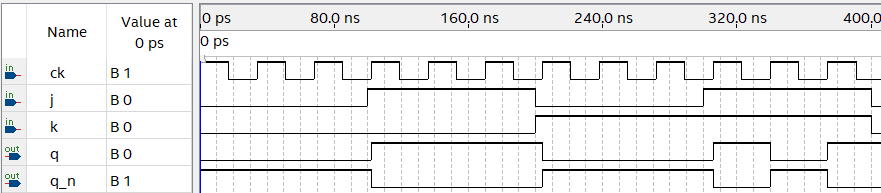
\includegraphics[width=0.95\linewidth]{imgs/jk_wave}
	\caption{Временная диаграмма для JK-триггера}
	\label{fig:jk_wave}
\end{figure}


\subsection{T-триггер}

%\VerbatimInput{../t_latch.v}

\begin{table}[]
	\begin{center}
		\begin{flushleft}
			\tablecaption{Таблица переходов для T-триггера}
		\end{flushleft}
		\label{tab:t_flip_flop}
		\begin{tabular}{|c|c|}
			\hline
			$T$ & $Q$                   \\ \hline
			0   & $Q_{prev}$            \\ \hline
			1   & $\overline{Q_{prev}}$ \\ \hline
		\end{tabular}
	\end{center}
\end{table}

\subsection{Измененный D-триггер}

%\VerbatimInput{../d_latch.v}

% Сравнение RTL

\subsection{Задний D-триггер}

%\VerbatimInput{../d_latch.v}

% Сравнение RTL

\subsection{Тестирование D-триггер}

\subsection{Тестирование JK-триггер}

\subsection{D-триггер с очисткой}

% Сравнение RTL

\subsection{D-триггер со сбросом}

% Сравнение RTL

\subsection{Какая то ересь в №10}

% Сравнение RTL

\subsection{Какая то ересь в №11}

% Сравнение RTL

\section{Контрольные вопросы}

\begin{enumerate}
	\item b) D-тpиrrep;
	\item AZ, BY, CX;
	\item Задержка распространения: $t_{pd}$ = максимальная задержка от входа к выходу;
	\item Синхронные триггеры позволяют изменять значение своего состояния только при подаче специального сигнала.
	Асинхронные могут изменять свое состояние в любой момент времени;
	\item Запрещенная комбинация -- комбинация входных сигналов, подача которых на вход триггера приведет его в неопределенное состояние;
	При подаче запрещенной комбинации на обоих выходах триггера будет низкий логический сигнал, при чем триггер установится в определенное состояние при подаче другого сигнала;
	\item D-триггер синхронный, в отличии от D-защелки, т.е. обновляет свое значение только при подаче сигнала;
	\item В схеме slave-master используется две D-защелки, когда схема на бистабильных ячейках более сложная и состоит из нескольких логических элементов с обратными связями;
	\item Время установки -- это время перед приходом перепада сигнала CLK, в течение которого сигнал D должен быть стабилен;
	\item Время удержания -- это время, в течение которого сигнал D должен быть стабилен, после прихода перепада сигнала CLK;
	\item На JК-триггер можно реализовать D-триггер и T-триггер;
	\item Разработайте схему Т-триггера на основе D-триггера (рис. \ref{fig:self_made_t_on_d});
	\begin{figure}[H]
		\centering
		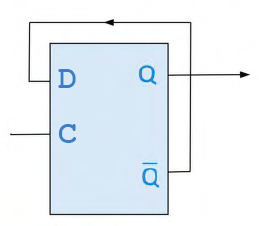
\includegraphics[width=0.6\linewidth]{imgs/self_made_t_on_d}
		\caption{Т-триггера на основе D-триггера}
		\label{fig:self_made_t_on_d}
	\end{figure}
	\item Операторы непрерывного присваивания на языке Verilog соединяет сигналы внутри схемы;
	\item Блокирующие присваивания выполняются последовательно, один за другим.
	Неблокирующие присваивания выполняются одновременно;
	\item Синхронный сброс может произойти только по фронту синхронизирующего сигнала, в то время как асинхронный сброс может произойти в любой момент времени;

	Пример синхронизирующего сброса:
	\begin{verbatim}
	module dff_sync_rst_n
	(	
		input clk,
		input rst_n,
		input d,
		output reg q
	) ;
	always @ (posedge clk)
		if (!rst_n)
			q <= О;
		else
			q <= d;
	endmodule
	\end{verbatim}
	
	\item Ключеве слова parameter в языке Verilog позволяет переиспользовать исходный код при разработке модулей разной разрядности. 
	С помощью данного параметра можно настраивать размерность модулей;
	\item $ P = \alpha C U^2 f$;
	
	$\alpha$ -- среднее число переключений в течении тактового периода;
	
	$C$ -- емкость нагрузки;
	
	$U$ -- напряжение питания;
	
	$f$ -- частота тактового сигнала;
	
	\item Ячейка блокировки -- ячейка, которая блокирует изменения состояния неиспользуемых элементов. 
	Данная ячейка применяется для снижения энергопотребления логического элемента;
	\item Блокировка тактового сигнала может привести к появлению шумов в линии тактового сигнала и ложного срабатывания управляемого элемента.
\end{enumerate}

\section{Выводы по работе}

В ходе работы получен опыт проектирования схем в программе Quartus с помощью языка Verilog.
Полученное устройство было протестировано с помощью бенчтестов в программе Quartus Simulation Waveform editor.
В процессе работы были смоделированы различные триггеры с синхронной и асинхронным управлением, сигналами сброса.
В процессе был получен опыт работы с платой DE10-Lite, на которой проверялась работоспособность полученного устройства.

\newpage 
\renewcommand{\refname}{{\normalsize Список использованных источников}} 
\centering 
\begin{thebibliography}{9} 
	\addcontentsline{toc}{section}{\refname} 
	\bibitem{Verilog} Thomas D., Moorby P. The Verilog Hardware Description Language. – Springer Science \& Business Media, 2008.
	\bibitem{citekey} Khor W. Y. et al. Evaluation of FPGA Based QSPI Flash Access Using Partial Reconfiguration //2019 7th International Conference on Smart Computing \& Communications (ICSCC). – IEEE, 2019. – С. 1-5
\end{thebibliography}

\end{document} % конец документа






